\section{Software preparation\label{softwarePreparation}}

\subsection{Data structures and file formats}
Two types of data files are mainly used in this project: an input file, specifying the bodies,
their geometry and initial configuration in a scene, and an output file for the simulation
results.

\subsubsection{Input data}
The input data has a graph structure which is visually represented in figure~\ref{sceneSchema}.
Geometric objects are represented as \emph{meshes} of triangles. (Polygons with a larger number of
sides must first be split into triangles; this is always possible~\cite{Skiena:98}.) Each triangle
(or \emph{face}) of the object's surface is delimited by three \emph{vertices}. To make the
geometric algorithms work nicely, we also require the mesh to be closed (to have a well-defined
interior) and contain no unnecessary triangles on its inside; in other words, it must describe the
surface of a polyhedron. This simple structure is sufficient to represent a great variety of
shapes, and although a large number of vertices is necessary to adequately approximate curved
surfaces, the ease of handling this data outweighs the costs caused by its quantity.

\begin{figure}
\centerline{\scalebox{0.35}{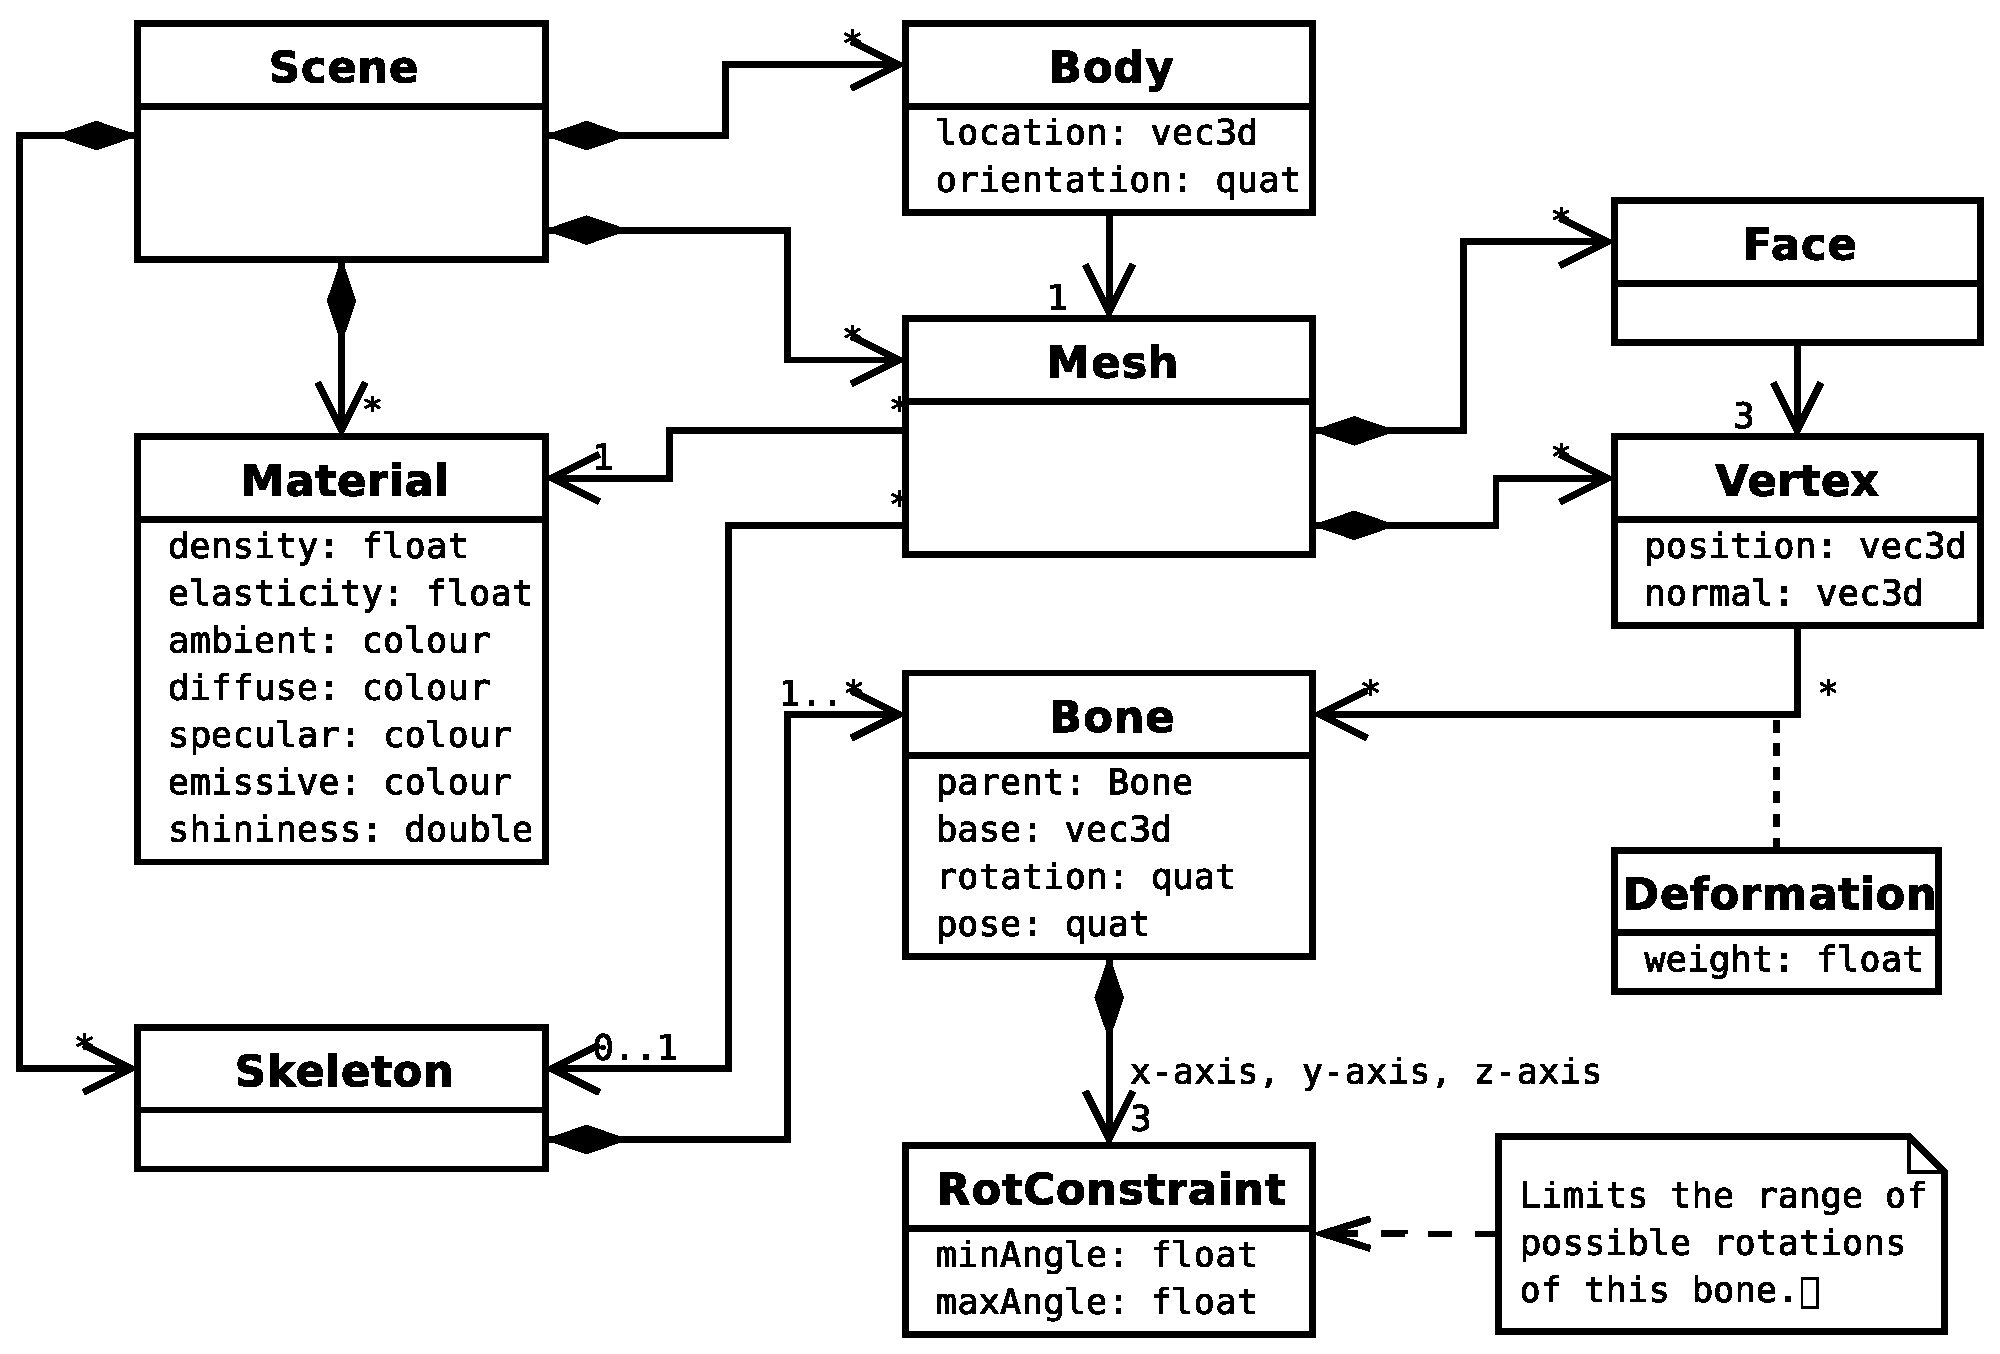
\includegraphics{figures/schema}}}
\caption{Structure of the input data to a simulation, using UML syntax.\label{sceneSchema}}
\end{figure}

Several \emph{bodies} in the scene may share the same mesh if they are identical up to rotation
and translation. A mesh is also associated with a \emph{material} which is used to determine the
visual rendering (colour) and the physical behaviour (density, elasticity).

If the scene contains articulated bodies, \emph{skeletons} must be defined in the file. A skeleton
is a tree of \emph{bones} in which each bone has an offset and a rotation relative to its parent.
If one bone~-- say an upper arm~-- in this structure moves while all other relative rotations stay
unchanged, then all children of this bone~-- up to the tip of the little finger~-- will be rotated
equally. This matches the natural behaviour of a skeleton. There can also be limits on the maximum
angles of rotation for each joint; these are discussed in more detail later in
section~\ref{generalizedCollisions}.

In an articulated mesh, each vertex is associated with one or more bones of a particular skeleton.
Normally it will be associated with one bone, but a weighted sum of two or even three adjacent
bones' transformations may be used to create the illusion of smoothly deforming joints. Hence it
is not possible to completely decompose an articulated body into its individual limbs, but the
articulated mesh must be treated as a whole.

Since this data structure is designed to be very general-purpose, I wanted to use a file format
which could easily be generated by 3D modelling applications or manually edited. I chose to use
\textsl{XML}\footnote{eXtensible Markup Language, \texttt{http://www.w3.org/XML/}} as a basis
since it is easy to read both by humans and by \textsl{XML} parsing libraries. I could not
find a format which suited my needs~-- all existing formats are either far too
complicated\footnote{for example X3D, \texttt{http://www.web3d.org/}} or not
powerful enough~-- and therefore designed a custom schema. I created scenes in this format by
modelling them in \textsl{Blender} (see below) and exporting them to the
\textsl{Cal3D}\footnote{Character Animation Library, \texttt{http://cal3d.sourceforge.net/}}
format; since \textsl{Cal3D} contains less information than required by the simulation, I could
semi-automatically convert it to my format using an
\textsl{XSLT}\footnote{eXtensible Stylesheet Language with Transformations,
\texttt{http://www.w3.org/TR/xslt}} stylesheet, and then add the missing information manually.

\subsubsection{Output data}
The output of a simulation is much simpler than the input data: All that is required is the
position and orientation, and possibly the velocities, of each body at each time step. For
articulated bodies, the orientation of each bone is also required. This suggests a simple
matrix layout in which bodies and bones are sorted along one dimension and time along
the other.

The output file is such a matrix, arranged in a simple \textsc{ascii} file format which can
directly be imported by \textsl{Octave} (see below). \textsl{Octave} can then be used for further
processing or evaluation of the results.

\subsection{Tools\label{softwareTools}}
\subsubsection{Programming languages}
I chose \textsl{Java~1.5}\footnote{Using Sun's J2SE JDK~5.0, \texttt{http://java.sun.com/}}
as language for the implementation of the bulk of the project. \textsl{Java}'s strictly
object-oriented paradigm and its package concept facilitate the management of large software
engineering projects; it is mature, well supported and benefits from an extensive run-time library.
I particularly appreciate its good type safety (and hence bug prevention) compared to languages
like \textsl{C}. I also make heavy use of the \emph{generic} type polymorphism added in
version~1.5.

\textsl{Java} is a verbose language though, so I decided that it would be beneficial to prototype
the algorithmically tricky parts in a concise language first. For this I used
\textsl{GNU Octave}\footnote{GNU Octave~-- \texttt{http://www.octave.org/}~-- uses a language
mostly compatible to \textsc{Matlab}~-- \texttt{http://www.mathworks.com/products/matlab/}},
a scripting language optimized for numerical computation on matrices and vectors. I implemented
almost all numerical algorithms in this project in \textsl{Octave} first; this version was too
slow to be of much practical use, but turned out to be extremely useful to guide the subsequent
\textsl{Java} implementation. Octave was also used for processing of simulation output, for
example to generate plots of the simulation behaviour.

\subsubsection{Libraries}
Rendered output is specified in the project requirements, and the most common choice for
displaying 3D graphics in \textsl{Java} programs is the
\textsl{Java3D}\footnote{\texttt{https://java3d.dev.java.net/}} library. \textsl{Java3D} provides
a clean object-oriented interface to either a software renderer or accelerated graphics hardware,
and is also quite well documented.

Processing of the input file was done using an \textsl{XML data binding tool} which I had
developed independently in summer 2005. This tool takes a grammar for an \textsl{XML} schema in
\textsl{RELAX NG}\footnote{\texttt{http://www.relaxng.org/}} format and generates a set of
\textsl{Java} classes implementing a run-time representation of that schema. The actual low-level parsing
is done by the \textsl{SAX}\footnote{Simple API for XML, \texttt{http://www.saxproject.org/}}
parser implementation in \textsl{Xerces}\footnote{Apache Xerces2 Java,
\texttt{http://xerces.apache.org/xerces2-j/}}.

Some of the numerical algorithms required by the simulation could have been obtained through
libraries. However, none of them are particularly complicated~-- their C implementation
in~\cite{NRinC} is at most a few pages long and is easy to translate into \textsl{Java}. I
therefore chose to implement the algorithms myself, giving me the freedom to combine them
intimately (see section~\ref{algorithmImplementation}).

\subsubsection{Tool chain}
For \textsl{Java} development, I set up the \textsl{Eclipse}\footnote{\texttt{http://www.eclipse.org/}}
environment, and a dual build system using the \textsl{Ant}\footnote{\texttt{http://ant.apache.org/}}
tool was kept as fallback in case of problems with \textsl{Eclipse}. To analyse the run-time
performance of the \textsl{Java} implementation,
\textsl{EJP}\footnote{Extensible Java Profiler, \texttt{http://ejp.sourceforge.org/}} was used.

I created input data for the simulation using \textsl{Blender}\footnote{\texttt{http://www.blender.org/}},
an open source 3D modelling/animation/rendering application. \textsl{Blender} supports internal
scripting in \textsl{Python}\footnote{\texttt{http://www.python.org/}} to extend its functionality.
This allowed me to write some short \textsl{Python} scripts which imported the results of a
simulation as an animation back into \textsl{Blender}, acting on the original models. This was useful
to review simulation results separately from the internal \textsl{Java3D} output. \textsl{Blender}
can also export animations to the \textsl{YafRay}\footnote{\texttt{http://www.yafray.org/}}
raytracer to produce high-quality video files. These AVI files were converted to MPEG-1 video
streams using \textsl{FFmpeg}\footnote{\texttt{http://ffmpeg.sourceforge.net/}}.

Some types of constraint involve very messy algebraic expressions
(appendix~\ref{constraintAppendix}). I found it useful to automatically generate optimized source
code implementing these expressions using
\textsl{Maple}\footnote{\texttt{http://www.maplesoft.com/products/maple/}}.

\subsubsection{Backup strategy}
All work was done either on PWF machines or my own computer. All project files were kept under
version control using \textsl{CVS}\footnote{\texttt{http://www.nongnu.org/cvs/}}, and regular
snapshots of the whole repository were transferred to the \textsl{Pelican} backup service.
A working build environment was maintained both on the PWF and my computer so that work could
continue seamlessly in case of disaster.

\subsubsection{Example scenes}
\begin{figure}
\centerline{
    \raisebox{2mm}{\scalebox{0.72}{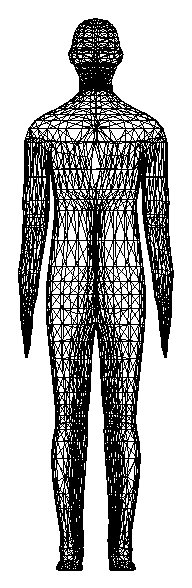
\includegraphics{figures/alfred-mesh}}}\hspace{1.3cm}
    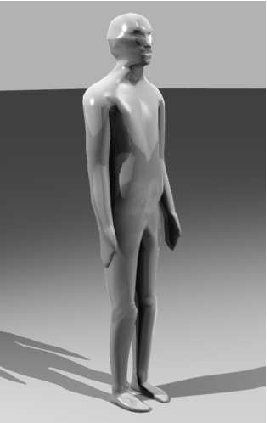
\includegraphics{figures/alfred-rendered}
    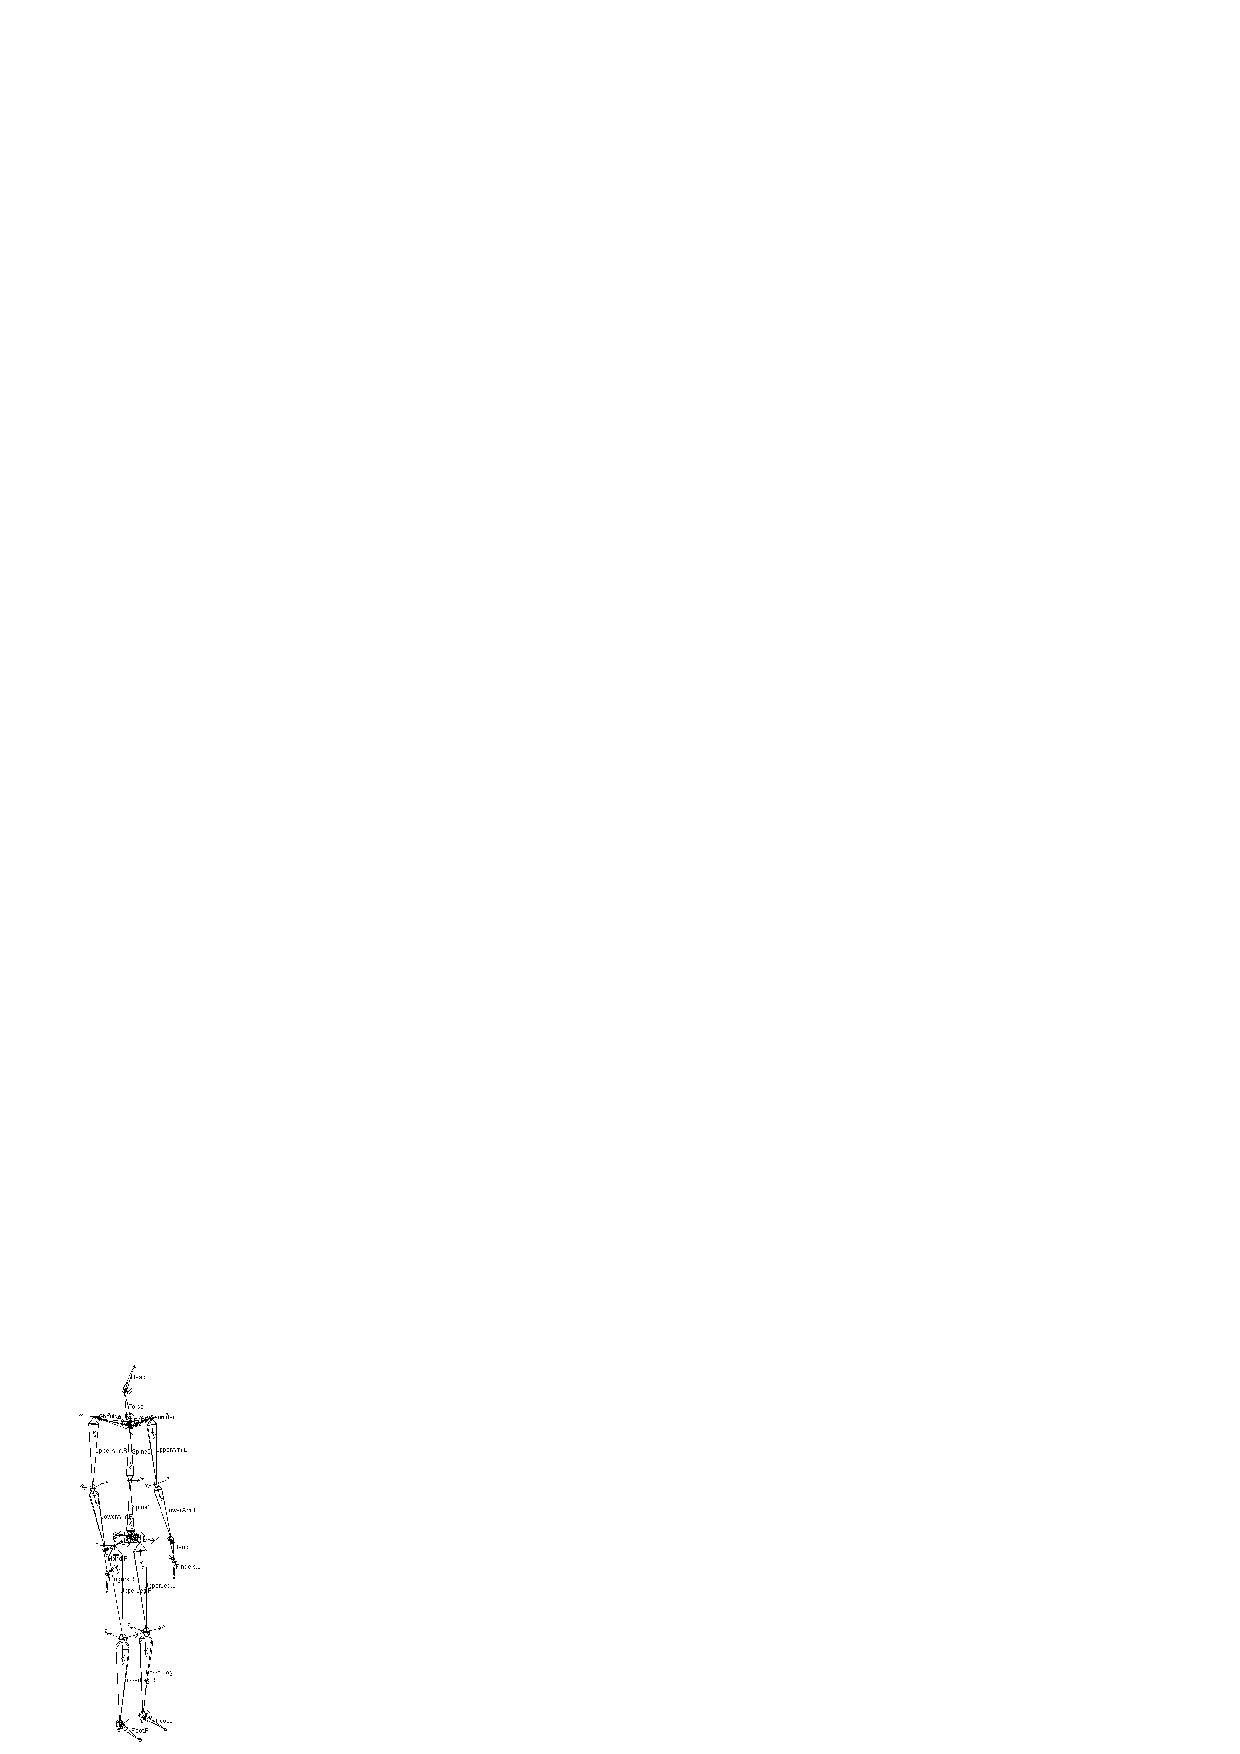
\includegraphics[width=45.16mm,height=71.6mm]{figures/alfred-skeleton}}
\caption{Alfred, one of the meshes used as input data. From left to right: The triangle mesh in
    wire-frame view; a raytraced perspective view; and the skeleton in its rest position.
    \label{alfredFigure}}
\end{figure}
I modelled all input data for the simulations in \textsl{Blender}. The most interesting mesh
is that of \emph{Alfred}, a humanoid articulated body (figure~\ref{alfredFigure}), which I created
using human anatomical data~\cite{Anatomy:03}. It has 2295 vertices, 4524 faces and is bound to
a skeleton of 25 bones, also shown in figure~\ref{alfredFigure}. There are some bugs in this
mesh~-- for example, strange cracks appear at the shoulders when the arms are lifted high~-- but
since creating good example data is not a primary objective of this project, these problems
should be disregarded.

\subsubsection{Dissertation}
\LaTeX{} was the definite choice for writing this dissertation because of its reliability,
good handling of cross-references, beautiful layout and many other benefits. I created the
figures using \textsl{Dia}\footnote{\texttt{http://www.gnome.org/projects/dia/}},
\textsl{Gnuplot}\footnote{\texttt{http://www.gnuplot.info/}} and the
\textsl{GIMP}\footnote{\texttt{http://www.gimp.org/}}.
